\documentclass[border=0pt]{standalone}
\usepackage{amsmath, amssymb}

%%font
\usepackage{euler}
\usepackage[OT1]{eulervm}
\renewcommand{\rmdefault}{pplx}

\usepackage{tikz}
\tikzset{every node/.style={draw, circle, inner sep=3pt}}
\usetikzlibrary{arrows}

\newcommand{\bx}{\mathbf{x}}

\parindent=0pt

\begin{document}
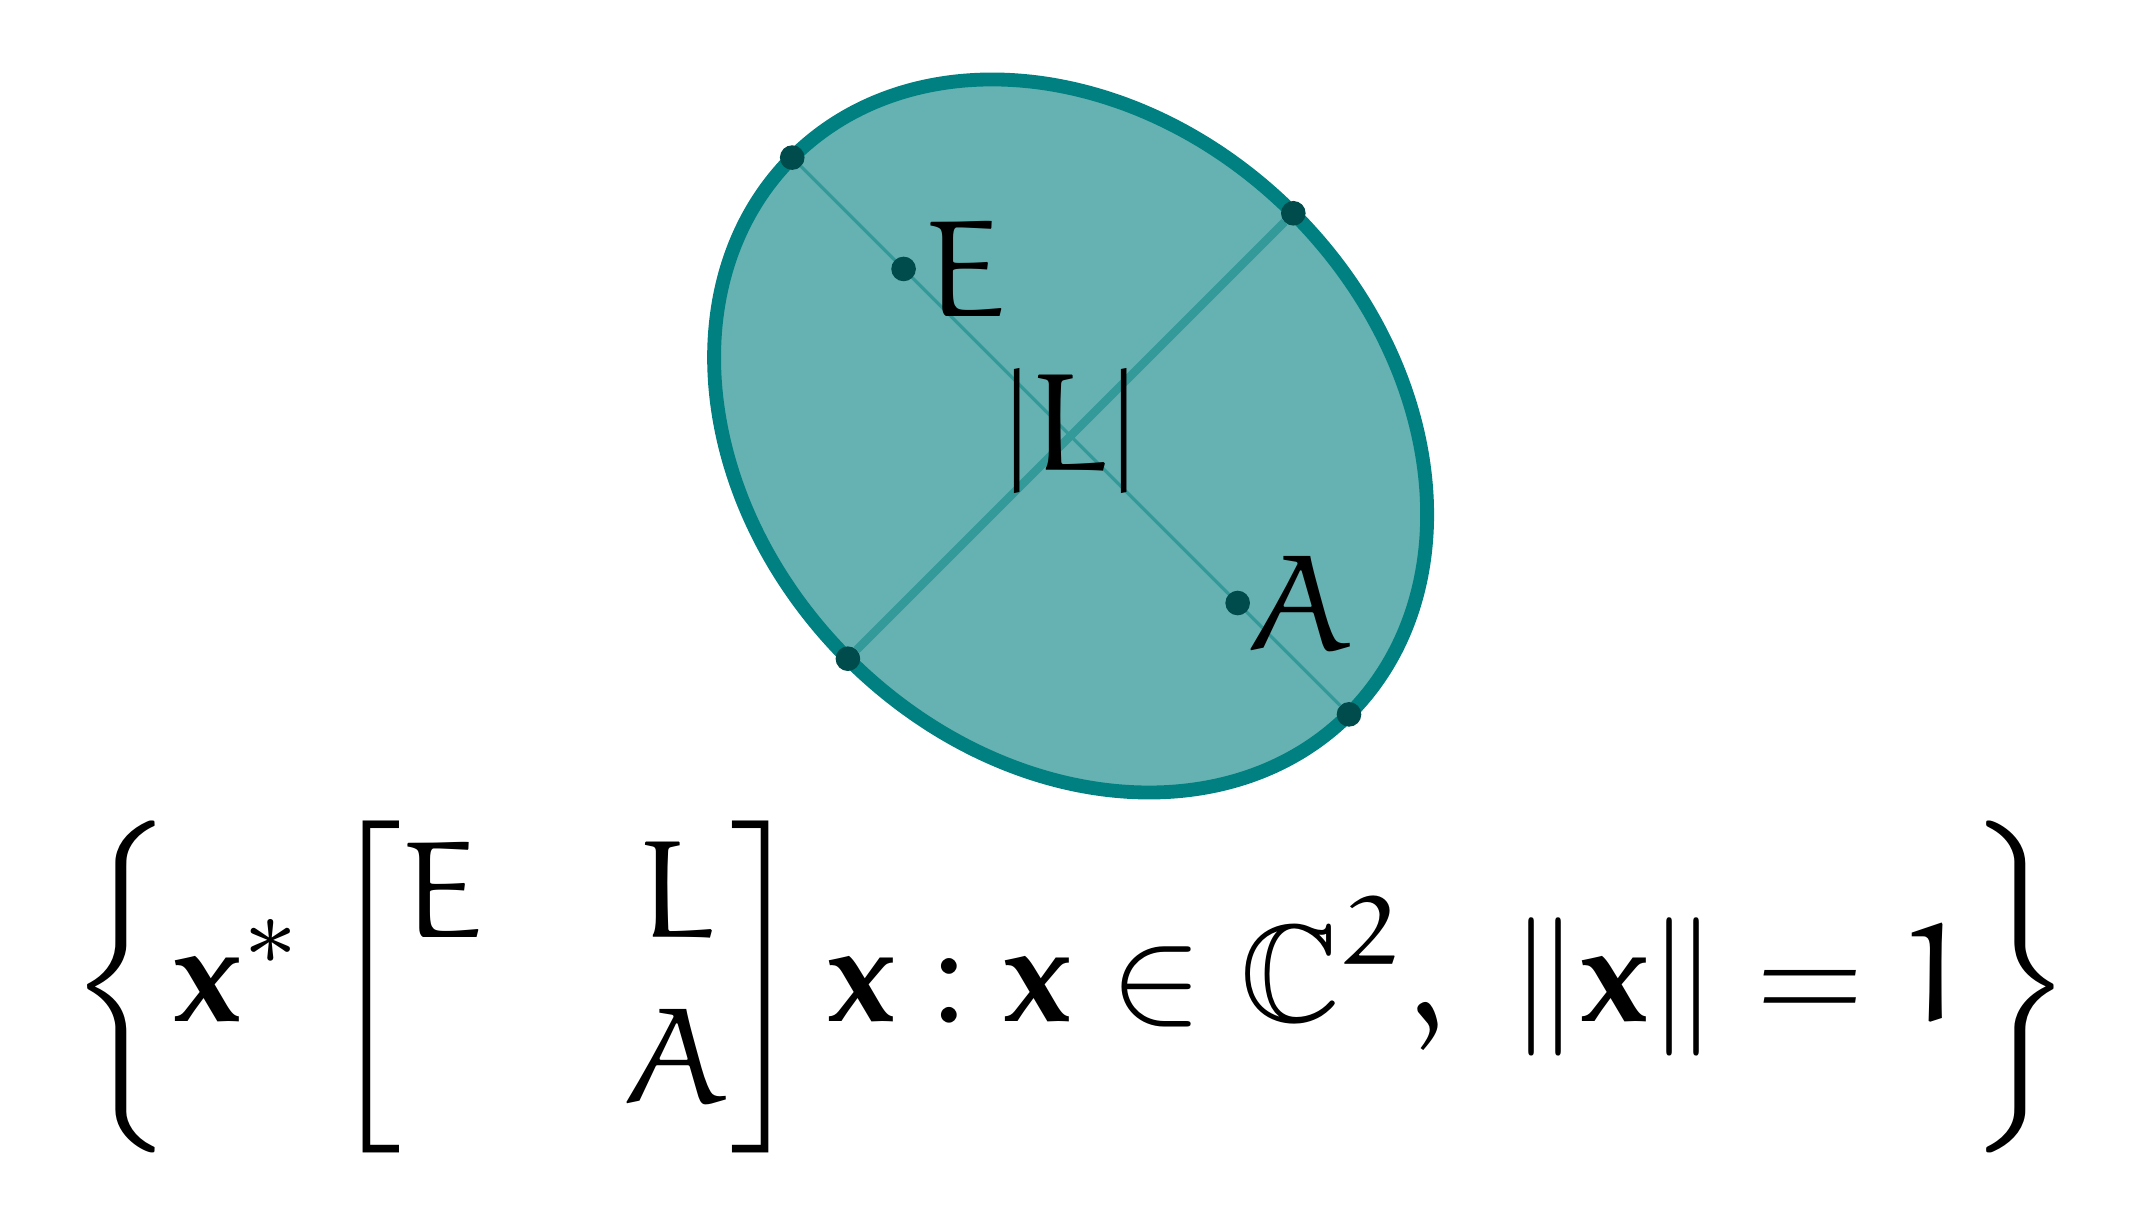
\begin{tikzpicture}
\draw[draw=teal, line width=5pt, fill=teal!60, rotate=-45] (0,0) ellipse (5cm and 4cm);

\begin{scope}[every node/.append style={draw=black!40!teal, fill=black!40!teal}]
\node (l1) at (135:5) {};
\node (l2) at (-45:5) {};
\node (s1) at (45:4) {};
\node (s2) at (225:4) {};
\draw[teal!80, very thick] (l1) -- (l2);
\draw[teal!80, line width=3pt] (s1) -- (s2);


\node (f1) at (135:3) {};
\node (f2) at (-45:3) {};
\end{scope}

\node[draw=none, rectangle, xshift=0.8cm, scale=5] at (f1.center) {$E$};
\node[draw=none, rectangle, scale=5] at (0,0) {$|L|$};
\node[draw=none, rectangle, xshift=0.8cm, scale=5] at (f2.center) {$A$};

\node[draw=none, rectangle, scale=5] at (0,-7) {$\displaystyle\left\{ 
    \bx^* \begin{bmatrix} E & L \\ ~ & A \end{bmatrix} \bx : 
    \bx\in\mathbb{C}^2,\ \|\bx\| = 1
\right\}$};






  

\end{tikzpicture}
\end{document}
